\section{Ein Beispiel zum nachrechnen und -bauen}

\begin{frame}{Das System}
  \begin{figure}
    \caption{Eine Hand kann in das System gehalten werden und der Hintergrund ist weiterhin zu sehen.}
    \centering
    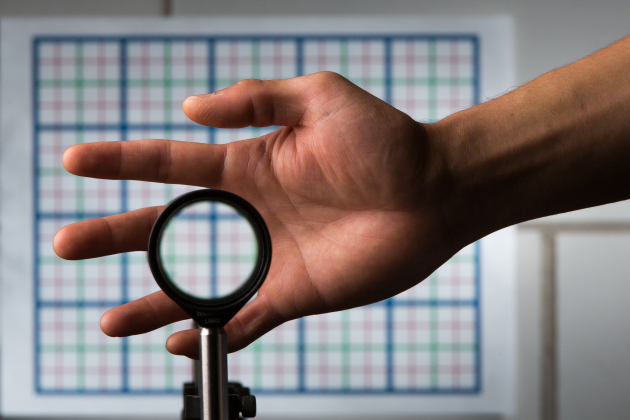
\includegraphics[height=0.6\textheight]{images/hand-cloak.jpg}
  \end{figure}
  Die folgenden Folien beziehen sich auf
  \href{https://www.rochester.edu/newscenter/watch-rochester-cloak-uses-ordinary-lenses-to-hide-objects-across-continuous-range-of-angles-70592/}{diese Veröffentlichung}
  von Howell und Choi der Universität Rochester aus dem Jahr 2014.
\end{frame}

\begin{frame}{Matrizenoptik}
  \begin{columns}
    \begin{column}{0.48\textwidth}
      \begin{figure}
        \centering
        \caption{Das System in Seitenansicht.}
        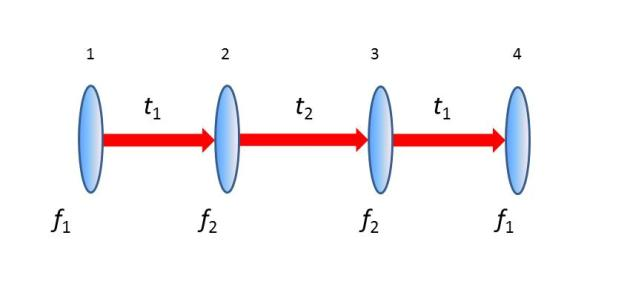
\includegraphics[width=\textwidth]{images/linsen.jpg}
      \end{figure}
    \end{column}
    \begin{column}{0.48\textwidth}
      D\"unne Linse
      \begin{align}
        F_i &=
        \begin{pmatrix}
          1 & 0 \\
          -\frac{1}{f_i} & 1 \\
        \end{pmatrix}
        \intertext{Translation}
        T_i &=
        \begin{pmatrix}
          1 & t_i \\
          0 & 1 \\
        \end{pmatrix}
      \end{align}
    \end{column}
  \end{columns}
\end{frame}

\begin{frame}{Warum vier Linsen?}
  Eine Tarnkappe der L\"ange $L$ wird in der Matrizenoptik durch
  \begin{align}
    M_\text{tarn} &=
    \begin{pmatrix}
      1 & L \\
      0 & 1 \\
    \end{pmatrix}
    =
    \begin{pmatrix}
      A & B \\
      C & D \\
    \end{pmatrix}
    \intertext{dargestellt. Eine Linse kann diese Bedingung nur erfüllen, wenn}
    M_{L=1} &=
    \begin{pmatrix}
      1 & 0 \\
      -\frac{1}{f_1} & 1 \\
    \end{pmatrix} = M_\text{tarn}
    \intertext{gilt, also}
    f_1 &\to \infty\:.
  \end{align}
  Das entspricht einer Glasscheibe.
\end{frame}

\begin{frame}{Zwei Linsen}
  Die Gleichung f\"ur zwei Linsen lautet
  \begin{align}
    M_{L=2} &= F_2\:T_1\:F_1 =
    \begin{pmatrix}
      1-\frac{t_1}{f_1} & t_1 \\
      -\frac{f_1+f_2-t_1}{f_1f_2} & 1-\frac{t_1}{f_2} \\
    \end{pmatrix} \stackrel{!}{=}
    \begin{pmatrix}
      1 & L \\
      0 & 1 \\
    \end{pmatrix}
    \intertext{Daraus folgt}
    \begin{drcases}
      t_1 = L = 0 \\
      f_1 \to \infty \\
      f_2 \to \infty
    \end{drcases}
    &=
    \begin{pmatrix}
      1 & 0 \\
      0 & 1 \\
    \end{pmatrix}
  \end{align}
\end{frame}

\begin{frame}{Erweiterung auf drei Linsen}
  \begin{align}
    M_{L=3} = F_3\:T_2\:M_{L=2} &=
    \begin{pmatrix}
      \frac{f_1f_2-t_1f_2-t_2f_2-t_2f_1+t_1t_2}{f_2} & t_1f_2-t_1t_2+t_2f_2 \\
      -\frac{f_1f_2+f_2f_3-t_1f_2-t_2f_2+f_1f_3-t_1f_3-t_2f_1+t_1t_2}{f_1f_3}
      & \frac{f_2f_3-t_1f_3-t_1f_2-t_2f_2+t_1t_2}{f_3} \\
    \end{pmatrix}
    \intertext{Es ergeben sich durch die Bedingungen einer Tarnkappe:}
    C &= 0 \\
    f_2 &= -\frac{(f_3-t_2)(f_1-t_1)}{1}
  \end{align}
\end{frame}
